\documentclass[a4paper,11pt]{article}
\usepackage[utf8]{inputenc}
\usepackage[spanish]{babel}
\usepackage{natbib}
\usepackage{parskip}
\usepackage{graphicx}
 
\title{La influencia de los jugadores de videojuegos online en las estrategias publicitarias de las marcas. Comparativa entre España y Corea} 
\author{\LARGE Johnny Bajaña Zajia\\ \texttt{jbajana@correo.ugr.es}} 

\begin{document}\maketitle 

RESUMEN\\
El negocio de los eGames (videojuegos online) en España ha conseguido más de 1,8 billones de euros de beneficio en el año 2016. La publicidad no es ajena al potencial de este mercado y las marcas estudian cuáles son las mejores formas de acercarse y adaptarse al entorno de los eGames. En el presente trabajo se analizan las estrategias publicitarias más eficaces para las marcas en el mundo de los videojuegos en red. Para ello, se han investigado a los jugadores (eGamers) a través de una encuesta de 60 preguntas que abordaban cuestiones como hábitos lúdicos, visionado de publicidad en los juegos, compra de artículos anunciados o publicidad en competiciones. El mismo cuestionario se ha realizado tanto a jugadores coreanos, ya que la industria de los video-juegos en Corea del Sur es la más avanzada del mundo, como a jugadores españoles, al ser España el cuarto país europeo en eGames y ser nuestro objeto de estudio. Tras la investigación, algunos de los resultados más relevantes indican que la publicidad online convencional no llama la atención a los consumidores «gamers» y se determina que la mejor estrategia se basaría en la presencia de marca a través de productos prescritos o utilizados por los «gamers» profesionales, ya que los espectadores, a la vez que ven las partidas, observan qué elementos usan los jugadores.

ABSTRACT\\
The eGames business (online video games) in Spain generated more than 1.8 trillion euros in profits in 2016. Advertising is no stranger to the potential of this market, and brands study the best ways of approaching and adapting to the world of eGames. In this report, we analyze which the most effective advertising strategies for brands in the online video game world are. To do this, the players (eGamers) answered a 60 question survey that addressed issues such as playful habits, the viewing of advertisements in games, the purchase of advertised items and advertising in competitions. Korean and Spanish players answered the same questionnaire considering that South Korea has the most advanced video game industry in the world and Spain is the fourth European country in eGames and our subject of study. After the investigation, some of the most relevant results indicate that conventional online advertising does not attract the attention of gamers as consumers. We determined that the best strategy would be based on brand presence through products that are prescribed or used by professional gamers, since spectators, as they watch the games, also observe what elements and accessories the players use.

PALABRAS CLAVE | KEYWORDS\\
Videojuegos en red, deportes electrónicos, publicidad en videojuegos, contenidos de marca, estrategias, publicidad, jugador español, jugador coreano.\\
eGames, eSports, advergame, branded content, strategies, advertising, Spanish gamer, Korean gamer.

\section{Introducción y estado de la cuestión}
Los videojuegos han obtenido más de 200 millones de dólares de beneficio por patrocinios y más de 150 millo- nes por publicidad convencional, según datos obtenidos en el 2017 «Global Games Market per Region» realizado por Newzoo (2016a) y basado en datos de 2016 (Newzoo es el proveedor líder de inteligencia de mercado que abarca los juegos globales, eSports y mercados móviles, con investigaciones en el ámbito de los videojuegos), que además afirma en su 2017 «Global Esports Market Report» (\cite{VALENTINA2016}) que el «gaming» es uno de los pasatiempos favoritos de los «millennials» (jóvenes nacidos a partir de los años 80; esa «complicada» audiencia que las marcas ansían conquistar).\\ 
En el negocio de los videojuegos siempre ha estado presente la publicidad. No obstante, es durante estas dos últimas décadas cuando el «juego», por el desarrollo y consolidación de Internet, ha evolucionado geométricamente y la publicidad debe adaptarse y ser consciente del potencial de negocio que esto conlleva (\cite{Pedrycz2016}). Son las propias marcas –ya sean medios de comunicación, plataformas, firmas de electrónica o telefonía– las que desde hace unos años están apostando por lo que hemos acuñado como los eGames (videojuegos electrónicos que se juegan online)\cite{Agarwal2016}.

\subsection{Los videojuegos en red (eGames) en España}

Estando en noveno lugar en el ranking mundial y en cuarto puesto con respecto al marco europeo –por detrás de Alemania, Reino Unido y Francia, en orden descendente de ingresos–, la industria de los videojuegos en red en España ha recaudado más de 1,8 billones de euros de beneficios en 2016 (Newzoo, 2017). Según el estudio del
«Infographic Spanish Games Market 2016», la población española contaba con 47,2 millones de personas de las cuales 36 millones eran internautas y 24 millones de ellos eran jugadores (gamers: personas que juegan a través del móvil, PC o dispositivos digitales análogos tipo consolas o tabletas). Y el 1º Observatorio de Deporte Electrónico en España 2016, realizado por Arena Media, afirma que: 1) 1 de cada 2 jugadores españoles gasta dinero en los eGames y no solo se lo descarga o juega online de forma gratuita; 2) El gasto promedio de jugador por año es de 130 euros;
3) 2 de cada 3 internautas en España juegan a algún tipo de videojuego en cualquier dispositivo.
Además, según el Libro Blanco del Desarrollo Español de Videojuegos 2016, realizado por DEV (Asociación Española de Empresas Productoras y Desarrolladoras de Videojuegos y Software de Entretenimiento), el 40\% de estos ingresos son gracias a diferentes fuentes alternativas, como el desarrollo de terceros, la venta de servicios y la formación. Sin embargo, establece que el 34\% de los ingresos provienen de la venta digital, es decir, videojuegos que se juegan de forma online. Y otro 10\%, de la publicidad en los videojuegos «free to play». Con estos datos podemos ver cómo la industria que antes se basaba en la venta física y la utilización de dispositivos como la PlayStation (anterior «reina» de los dispositivos para videojuegos) ahora ha cambiado y que el «nuevo rey» es Internet, con el ordenador como dispositivo estrella. La era digital se ha consolidado a pesar de que se sigan usando consolas, pero con conexión a Internet  \cite{Erik2015}.

Pero el uso de las pantallas y los videojuegos va más allá. En la actualidad, el consumo multipantalla o uso simultáneo de varios medios o dispositivos es una realidad que tenemos que asumir y aprovechar. En este sentido, hay que ser conscientes de que uno de cada tres jugadores alterna las cuatro pantallas (televisión, ordenador, tabletas y smartphones)\cite{Pedrycz2016}.

\subsection{Los deportes electrónicos (eSports) y los MMO juegos (MMO games)}
En la actualidad, la unión del PC u ordenador con la venta digital y la competición, dan lugar a los denominados eSports. Este término fue acuñado por el Instituto de Arena Media en 2016 en el 1º Observatorio del Deporte Electrónico en España. En este estudio, se utilizan las palabras «deporte electrónico» en el título, referidas a los eSports, por lo que en la propia cabecera ya nos dice que los eSports son las competiciones que se juegan a través de la pantalla del ordenador y/o consola.\\
Más allá de las audiencias, los deportes electrónicos tienen detrás unos valores que permiten a las marcas formar parte de este mundo para adherirse a ellos o reformar los de la marca, si son similares en valores. Estos juegos tienen un componente estratégico que atrae a personas con este tipo de habilidades que saben trabajar en equipo y que tienen dotes de liderazgo (\cite{Liu2015}). Además, estos juegos son vanguardistas en cuanto al diseño y al espectáculo que están dando. Por otro lado, la pieza fundamental del origen de los deportes electrónicos es la comunidad, dado que en sus inicios no contaba con grandes empresas que apoyaran estas competiciones de manera económica (\cite{Agarwal2016}).

\subsection{Estrategias publicitarias}
En el marco actual de la publicidad en el sector de los videojuegos en red en España, las principales tácticas que se patrocino y los contenidos de este país, el sector de los video-juegos en red (eGames) y los deportes electrónicos (eSports) está experimentando un gran avance, pero aún no existe un modelo de negocio a seguir. Lo bueno de este territorio para las marcas es que, al ser nuevo, las normas no están dictadas o asentadas, como puede ser en otros patrocinios deportivos. Por lo tanto, incita a una riqueza o abundancia mucho más importante por parte de las ligas o los equipos a hacer activaciones y entradas diferentes de las marcas \cite{Kesharwani2017}.

\subsection{La inversión en deportes electrónicos (eSports)}
El caso de Media Pro y la LVP es un claro ejemplo de cómo empresas españolas invierten en deportes electrónicos. La LVP o Liga de Videojuegos Profesional es una liga que nace nacionalmente queriendo exportar su modelo y reproducirse en otros países, y terminó siendo la liga nacional más grande a nivel europeo. El grupo audiovisual Media Pro compró la mayoría de las acciones de esta organizadora de ligas. Según declaraciones de LVP en rueda de prensa, esta inversión de casi 5 millo- nes de euros tiene el objetivo de «profesionalizar, expandir e impulsar la competición», contando con mayores recursos para los departamentos de marketing y patrocinios. Esto tiene un beneficio para profesionalizar la industria.  No obstante, esto sí pasa en Corea del Sur, con marcas como Samsung muy vinculadas en el inconsciente de la audiencia a los videojuegos en red por su famoso equipo «Samsung Galaxy White».\\
Sobre el mismo tema pero a la inversa, la empresa GAME, que se dedica a la venta de videojuegos en Gran Bretaña, fagocitó SocialNAT, una plataforma española en la que se retransmiten eSports. Aquí vemos como empresas del extranjero muestran interés y ven beneficios en el visionado de los deportes electrónicos en España (\cite{Erik2015}).


\section{Material y métodos}
Esta investigación partió con el objetivo general de analizar los videojuegos en red en España, así como el comportamiento de la industria y de la publicidad en los mismos. Como objetivos específicos, se pretendía definir el perfil del jugador español y su conducta ante la publicidad y las marcas aparecidas en los juegos y las competiciones. La comparativa con el jugador coreano se realizó con el objetivo de tener a éste último como referente del jugador avanzado (ya que Corea es el país con más seguidores de este tipo de juegos) y poder analizar qué estrategias publicitarias podrían ser más eficaces para este tipo de público objetivo y su posible aplicación a las estrategias publicita- rias de marcas dirigidas a un público español.\\
Con el objetivo de analizar cuáles son las estrategias publicitarias más eficaces para las marcas en el mundo de los videojuegos en red, se decidió investigar y comparar las rutinas de juego, el visionado de publicidad, los comportamientos de compra y la opinión de imagen de marca de jugadores españoles (nuestro objeto de estudio) y jugadores coreanos (donde la cultura del jugador en red está más asentada). Para realizar la investigación, se optó por la técnica del cuestionario online. El cuestionario es una técnica cuantitativa consistente en investigar una muestra de sujetos representativos de una población. Las ventajas de este método de recolección de datos son que permite obtener información de casi cualquier colectivo, además de que nos facilita la estandarización de los datos, es decir, podremos tratarlos informáticamente y analizarlos según estadísticas (\cite{Erik2015}). Se consideró que el mejor medio para alcanzar al universo objeto de estudio era Internet. Gracias al cuestionario online, se puede alcan- zar a un amplio número de personas con bajo coste. A su vez, esta herramienta permite interactuar con el entrevistado, lo que se traduce en menos preguntas incompletas.\\
La encuesta a jugadores coreanos fue exactamente igual que la pasada a los españoles y fue cumplimentada por un total de 293 jugadores.\\
Ambas encuestas fueron supervisadas y pre-testadas para su validación por expertos en metodologías científicas de investigación de la Universidad Jaume I y los resultados fueron volcados y cruzados para su análisis estadístico a través del programa SPSS versión 23.0 para el análisis y validación de los estadísticos básicos.
\section{Análisis y resultados}
Las 60 preguntas que se les han hecho a los jugadores españoles analizan el modo en el que estos consumen los videojuegos y las competiciones, cómo la publicidad es recibida por ellos, conocer cómo se está usando actualmente la publicidad y cuáles podrían ser los formatos publicitarios más eficaces. Seguidamente, exponemos y ana- lizamos algunos de los resultados más significativos obtenidos.\\
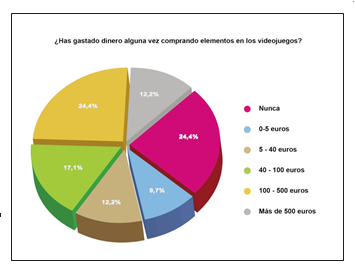
\includegraphics[scale=1]{FIGURA2.png} 
Respecto a las preguntas de la primera sección (hábito y tipo de juegos) más del 40\% juega a videojuegos todos los días y un 35\%, varios días a la semana. Se les preguntó sobre la categoría de videojuegos MMO a la que jugaban más, a lo que más de la mitad respondieron categoría «Shooter» (videojuegos de disparo), un 38\% a MOBA (video- juegos de batalla y estrategia colectiva) y un 35\% videojuegos de estrategia. Los porcentajes de esta pregunta suman más del 100\% ya que era de opción múltiple. En cuanto a la pregunta sobre si habían visto alguna vez una competición de deportes electrónicos, el 53\% de ellos contestaron afirmativamente.
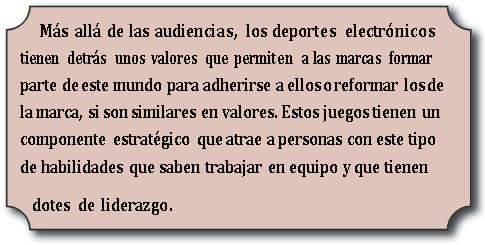
\includegraphics[scale=1]{FIGURA1.png} 
\subsection{Comparativa de los resultados entre los jugadores españoles y los surcoreanos}
En esta segunda encuesta hemos tomado una muestra similar, 293 encuestados con 60 preguntas por encuesta, examinando al público de la República de Corea del Sur.\\
En la primera sección, todos los encuestados afirman ser coreanos, con un porcentaje mayor de juego que el español, con un 40\% de ellos que juega varios días a la semana, y la mitad de todos ellos juega todos los días, por lo que la frecuencia de juego es mucho mayor en compara- ción a la española.\\
Casi todos los encuestados juegan a video-juegos MOBA (batalla en arena), dentro de los cuales se incluyen los videojuegos en red más famosos como «LoL», «War of Warcraft», y las otras categorías son ignoradas, a diferencia de los españoles en los que los encuestados se reparten de manera más equitativa en las categorías. Por último, una gran diferencia es que el 95\% de los encuestados han visto alguna vez una competición de deportes electrónicos, con respecto al 53\% español. En cuanto a la segunda sección sobre el com- portamiento de juego, el jugador coreano presenta una dedicación mucho mayor que el español con casi 80\% de los encuestados que dedica más de tres horas al día a videojuegos en contraste al 29\% español que dio la misma respuesta. En cuanto al horario, cambia totalmente, el 60\% de los coreanos afirma jugar en los descansos en el trabajo/universidad y un 25\%, entre las 8 y 12 de la mañana, a diferencia de la preferencia nocturna que se da en el español. El lugar de juego y el dispositivo utilizado es de las mayores diferencias entre ambos públicos, el coreano con un perfil más inclinado a jugar fuera de casa (94\% de respuesta) y con el móvil (82\%) y el español con un perfil más proclive a jugar dentro de casa (100\%) y utilizando el PC (57\%).

\begin{table}[htbp]
\begin{center}
\begin{tabular}{|l|l|}
\hline
Categoría & Porcentaje \\
\hline 
\hline Siempre & 50\% \\ 
\hline Casi siempre & 25\% \\ 
\hline Nunca & 25\% \\ 
\hline
\end{tabular}
\caption{Dinero gastado en compra de los videojuegos.}
\label{tabla:sencilla}
\end{center}
\end{table}

\section{Discusión y conclusiones}
Por lo tanto, una de las mejores estrategias en cuanto a publicidad para videojuegos sería la utilización de jugadores profesionales como factor de influencia al utilizar y prescribir productos y marcas. Serían embajadores de marca que generarían reconocimiento hacia la misma. El patrocinio de estos jugadores se basaría en la presencia de marca tanto durante el tiempo de partida como del visionado de competiciones de deportes electrónicos. Este patrocinio sería fundamental durante la retransmisión ya que los espectadores, a la vez que ven las partidas, observan qué elementos usan los jugadores, desde el teclado hasta la bebida que toman (\cite{Agarwal2016}).\\
Tras analizar y comparar las características de los jugadores españoles y coreanos en cuanto a su comportamiento de juego, visionado de publicidad, imagen de marca y comportamiento de compra, exponemos a continuación algunas de las conclusiones más significativas de nuestro estudio.
Gracias al aumento del público jugador de los deportes electrónicos las marcas que se vinculen estratégicamente con los videojuegos podrán beneficiarse de todo el potencial que los videojuegos en red y los deportes electrónicos ofrecen (competición, audiencia masiva, comunidad o fans) (\cite{Erik2015}). Como hemos visto, la publicidad online convencional no llama la atención a los consumidores jugadores, pero los productos prescritos por los jugadores profesionales son eficientes. Los jugadores aficionados se fían del criterio de los profesionales y, si bien  son críticos y saben que tener esos productos no les hará ganar las competiciones, declaran que saben que son pro- ductos de calidad. Esto se debe a un componente aspiracional. Por otro lado, el factor competitivo, que se incre- menta más aún en los jugadores surcoreanos, y el afán de superación personal hacen que quieran obtener mejores productos para alcanzar a sus «héroes» o modelos a seguir.\\

\section{Apoyos}
Este artículo se ha realizado con ayuda del proyecto de investigación titulado «El negocio publicitario en la sociedad digital: estructura de agencia, perfiles profesionales y nuevas tendencias creativas». Plan de Promoción a la Investigación de la Universidad Jaume I de Castellón. Código del proyecto P1-1B2015-27.

   
\bibliographystyle{apalike}
\bibliography{mybib}

\end{document}